%!TEX root = Tesi__Simone_Mariotti.tex
\chapter{Implementazione}
\fancyhead[R]{\bfseries Implementazione} 	
\fancyfoot[C]{\thepage }
\section {Android}
L'app per Android è stata sviluppata avendo come priorità la modularità. E' 
infatti molto semplice cambiare totalmente il comportamento del robot o la 
codifica dei messaggi sostituendo o modificando una singola classe senza 
coinvolgere il resto del codice.\\
La modularizzazione a grana più grossa è a livello di package\footnote{Un contenitore 
che racchiude classi che svolgono compitini affini}: ci sono tre package,
ognuno con un compito preciso, e sono \textbf{logic}, \textbf{messaging} e \textbf{opencv}.
\begin{figure}[H] \center
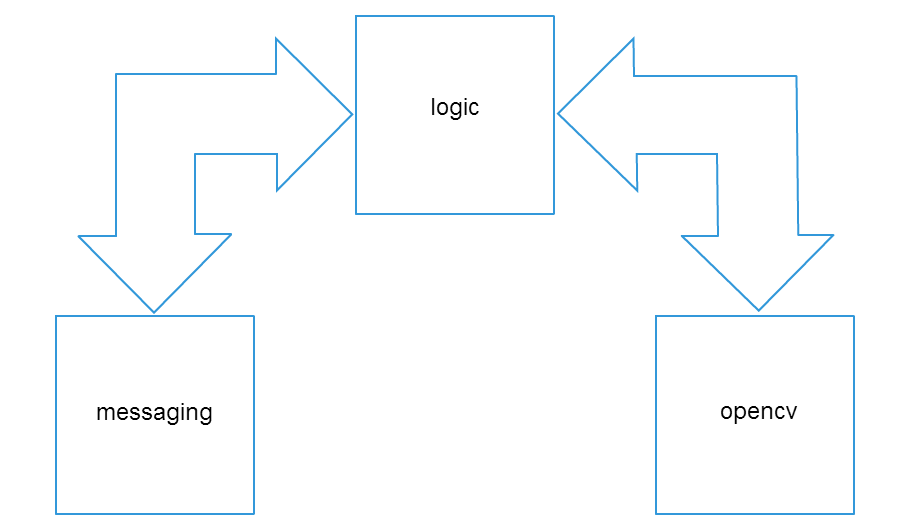
\includegraphics[scale=0.2]{immagini/package_diagram.png}
\caption{Schema di interconnessione dei package} 
\end{figure}
\subsection {Il package \textit{logic}}
Si occupa di reperire le informazioni dal mondo reale e analizzarle al fine di
eseguire l'azione più adatta.
Contiene tre classi: RobotActivity, RobotLogic e UpdateDirections.
\subsubsection{La classe \emph{RobotActivity}}
Come suggerisce il nome è l'Activity vera e propria, cioè quella classe che il 
sistema operativo istanzia all'avvio dell'app. Essa stessa istanzia e prepara tutti gli 
altri oggetti per l'esecuzione. Implementa due interfacce: View.OnTouchListener 
e CvCameraViewListener. 
La prima permette di gestire gli input da touch screen senza ricorrere ad una classe esterna,
la seconda è un'interfaccia presente nella libreria OpenCV e permette di ``intercettare''
i frame proveniente dalla camera prima che vengano renderizzati a schermo tramite 
l'override\footnote{Tecnica che permette di ridefinire il comportamento di un metodo 
ereditato} del metodo \textit{OnCameraFrame()}. Ogni frame verrà elaborato e solo alla
fine visualizzato a schermo.
All'avvio si occupa di inizializzare OpenCV tramite la 
callback \textit{BaseLoaderCallback} e ottiene il riferimento all'istanza dell'ADK
tramite l'ADKToolkit. E' buona norma interrompere le connessioni e liberare il canale usato 
nel momento in cui un'app viene chiusa. Per questo nel metodo \emph{onDestroy()} 
viene chiuso il canale usato per comunicare con Arduino tramite il metodo \emph{close()}
fornito dall'ADKToolkit.\\
In aggiunta alle normali funzioni di un'Activity RobotActivity integra un 
listner per gli eventi touch verificatesi all'interno della porzione di 
interfaccia utente che mostra il video proveniente dalla camera. Al verificarsi di un
tale evento viene invocato il metodo \emph{onTouch()} ereditato da View.OnTouchListener 
che esegue la media dei colori presenti in una regione di 8x8px intorno alle coordinate
in cui è avvenuto il tocco da parte dell'utente. Fornisce il colore così calcolato a 
alla classe TargetSearch del package \textbf{opencv} tramite il metodo pubblico 
di quest'ultima \emph{setTargetHsvColor()}. Questo sarà il colore che il robot cercherà
nella scena, il suo obbiettivo.

 \subsubsection{La classe \emph{UpdateDirections}}
 Questa classe è un ``singleton''\footnote{E' un design pattern descritto dalla 
 cosiddetta ``Gang of four'' nel libro ``Design Patterns''. 
 Permette la creazione di una sola istanza della classe e ne regola l'accesso. } 
 e si occupa di mostrare all'utente tramite  immagini e testi quello che  il 
 robot sta facendo o quale sarà la sua prossima  mossa. Dovendo agire 
 sull'UI\footnote{User Interface, interfaccia utente} deve essere eseguita sul thread
 che si occupa dell'UI, per questo implementa l'interfaccia \emph{Runnable} e 
 ogni sua esecuzione è lanciata  tramite \emph{runOnUiThread()}. 
 Le informazioni visualizzabili sono limitate e ben distinte,
 ad ognuna corrisponde un metodo da invocare per visualizzare quella data informazione
 a schermo. I metodi disponibili sono: 
 \begin{itemize}
 \item \emph{left()}: indica che l'obiettivo è visibile è stato individuato e si trova alla sinistra del robot.
 \item \emph{right()}: indica che l'obiettivo è visibile è stato individuato e si trova alla destra del robot.
 \item \emph{aimed()}: indica che l'obiettivo è visibile è stato individuato e si trova esattamente di fronte al robot che si muoverà in quella direzione.
 \item \emph{search()}: indica che l'obiettivo non è visibile, il robot si muoverà secondo l'algoritmo di ricerca.
 \item \emph{found()}: indica che l'obiettivo è visibile e il robot si trova a meno di 30 centrimetri.
 \item \emph{avoidingLeft()}: indica che è presente un ostacolo sul percorso del robot a meno di 30 centimetri. Il robot lo aggirerà verso sinistra. 
 \item \emph{avoidingRight()}: indica che è presente un ostacolo sul percorso del robot a meno di 30 centimetri. Il robot lo aggirerà verso destra.
 \item \emph{chooseColor()}: indica che il robot è in attesa che venga impostato il colore da cercare. 
 \end{itemize}
 La classe espone anche altri metodi che mostrano (\emph{show()}) o nascondono 
 (\emph{hide()}) la porzione di interfaccia che visualizza le indicazioni, oppure bloccano (\emph{lock()})
 e sbloccano (\emph{unlock()}) la possibilità di cambiare le indicazioni visualizzate.

\subsubsection{La classe \emph{RobotLogic}}
La classe \emph{RobotLogic} è il vero ``cervello'' di tutta l'app.\\
Viene chiamata in causa ogni volta che arriva un nuovo messaggio da Arduino. 
Per far questo si è usato un altro famoso design pattern, quello di ``Observable'' 
e ``Observer'' in cui l'``Observer'' è questa stessa classe e l'``Observable''
è la classe IncomingMessage del pacchetto \textbf{messaging}.\\
Alla ricezione di ogni messaggio viene invocato il metodo \emph{decodeMessage()}
che decodifica il messaggio ricevuto e crea un'istanza di DecodedMessage per 
accogliere le informazioni appena ricevute e facilitarne l'accesso. Se il messaggio
contiene informazioni sulla distanza del primo oggetto nella direzione del robot
allora tale distanza viene salvata nell'istanza in modo che successivamente si
possa usare per valutare in modo più preciso la situazione.\\
Il metodo principale della classe è \emph{think()} ed è invocato ogni volta che
dal package opencv, e in particolare dalla classe TargetSearch, giunge un aggiornamento
sull'obbiettivo, la sua eventuale presenza in scena e la sua posizione. \emph{think()}
viene effettivamente eseguito solo se sull'interfaccia utente è stato premuto "Start"
 e per prima cosa stabilisce in che fase l'iterazione precedente ha portato il sistema. \\
 Le possibilità sono:
	\begin{itemize}
	\item ``Cheer Phase'': indica che l'obbiettivo è stato trovato e il robot sta
	girando su se stesso per segnalare la fine della ricerca.
	\item ``Avoiding Phase'': indica che sulla traiettoria del robot si è presentato un ostacolo e lo sta aggirando. Si compone di tre sottofasi:
	\begin{itemize}
		\item Fase 1: scegliere in modo casuale una direzione tra destra e sinistra e ruota di circa 90° in quella direzione. 
		\item Fase 2: si muove in avanti per un tempo prestabilito.
		\item Fase 3: ruota di 90° nella direzione opposta a quella scelta nella fase 1.
	\end{itemize}
	\item ``Search Phase'': indica che l'obbiettivo non è stato ancora trovato e il robot si sta muovendo per trovarlo.
	\end{itemize}

Se si trova nella ``Cheer Phase'' ignora ogni comunicazione proveniente da 
Arduino, finisce la rotazione di segnalazione e invoca il metodo \emph{reset()} di 
RobotActivity per preparare il sistema all'inserimento di un nuovo obbiettivo da 
parte dell'utente.\\
Se si trova nella ``Avoiding Phase'' esegue in successione le tre fasi. 
Si può interrompere solo se durante le manovre di aggiramento dell'ostacolo
l'obbiettivo compare nella scena.\\
Se si trova nella ``Search Phase'' controlla se l'obbiettivo è presente in scena e 
si trova a meno di 30 centimetri, in caso di risposta affermativa ferma il robot,
interrompe l'esecuzione di \emph{think()} e attiva la ``Cheer Phase''. 
Se l'obbiettivo non è in vista ma c'è un oggetto a meno di 30 centimetri ferma il robot
e attiva la ``Avoiding Phase''.\\
Se l'obbiettivo non è visibile rimane in ``Search Phase'' e si muove in avanti.\\
Se l'obbiettivo è visibile ma si trova a più di 30 centimetri effettua le correzioni di rotta
necessarie per portarlo in direzione di marcia.\\
Se l'obbiettivo è precisamente di fronte al robot si muoverà in quella direzione.\\ 
La rotazione necessaria per portare l'obbiettivo esattamente di fronte al robot 
implica movimenti lenti e precisi che è difficile ottenere con i motori DC di cui è
fornito il robot. Lo scenario tipico è vedere i motori sforzarsi di muovere il robot
con un certo quantitativo di energia, aumentare quell'energia di un'unità e vedere 
il robot iniziare a ruotare velocemente. Purtroppo l'energia richiesta per 
mettere in rotazione il robot cambiava in funzione di troppe variabili: 
la direzione di rotazione, l'uso di entrambi i cingoli o solamente uno, 
la presenza di piccoli ostacoli sotto il robot. Per ovviare a questo problema che impediva 
una corretta movimentazione del robot quando erano necessari movimenti precisi 
si è usato una soluzione adattiva che permette al robot di trovare sempre la 
minima energia necessaria per muoversi. Per far questo il robot prende come riferimento 
la posizione dell'obbiettivo e tenta di ruotare, se all'iterazione successiva 
non nota uno spostamento relativamente all'obbiettivo allora aumenta 
l'energia inviata ad i motori. Appena si muove l'energia cessa di essere 
aumentata e il robot ruota in modo fluido e controllato.
\subsection {Il package \textit{opencv}}
Il package \textbf{opencv} è costituito di due sole classi. Si occupa di analizzare 
i frame proveniente dalla camera alla ricerca dell'obbiettivo, comunica poi la posizione 
dell'obbiettivo o l'assenza dello stesso alla classe RobotLogic del package 
\textbf{logic}.
\subsubsection{La classe \emph{ColorBlobDetector}}
\emph{ColorBlobDetector} è la classe che effettivamente cerca l'obbiettivo nei
frame proveniente dalla camera. L'obbiettivo gli viene fornito da RobotActivity 
tramite \emph{setTargetHsvColor()} nel momento in cui l'utente lo indica 
sull'interfaccia utente. I colori in OpenCV vengono rappresentati con un tipo di dato interno
detto Scalar che può essere assimilato ad un array. Il metodo che esegue 
l'operazione di ricerca è \emph{process()}. Per prima cosa converte lo schema di 
colori del frame sotto analisi da RGBa\footnote{Ogni colore è rappresentato da 
quattro valori compresi tra 0 e 255 per le immagini CV\_8U, cioè le immagini dove 
i colori sono memorizzati in un byte. I quattro canali sono R (red), G (green), 
B (blue) e a (alpha) }. a HSV\footnote{Ogni colore è rappresentato da quattro 
valori compresi tra 0 e 255 per le immagini CV\_8U, cioè le immagini dove 
i colori sono memorizzati in un byte. I quattro canali sono H (hue), S (saturation), 
V (value) e  a (alpha)} e filtra l'immagine in modo che rimangano solo 
i pixel che hanno un colore che si trova entro un certo intorno del colore cercato.
Usa poi la funzione fornita da OpenCV \emph{findContours()} che cerca i contorni delle
zone con il colore di nostro interesse e li restituisce come una un ArrayList di MatOfPoint;
MatOfPoint è un tipo di dato di OpenCV che è usato per memorizzare una quantità variabile
di punti che sono in relazione tra di loro, in questo caso dei punti che formano un contorno.
In seguito cerca il contorno che ha area maggiore e scarta tutti quelli che sono più piccoli 
del limite impostato ad un un'ordine di grandezza in meno. I contorni rimasti 
saranno quelli analizzati da TargetSearch.


\subsubsection{La classe \emph{TargetSearch}}
Questa classe per prima cosa invoca \emph{process()} di ColorBlobDetector passandogli
il frame da analizzare e raccoglie i risultati tramite \emph{getContours()} che restituisce 
i contorni individuati da \emph{process()}.\\
Scorre poi uno ad uno i contorni così ricevuti e trova per ognuno un ``Bounding Rectangle'', 
cioè il rettangolo di area minima che contiene per interno il contorno corrente, 
scartando tutti i rettangoli minori di un certo valore e mantenendo un riferimento 
a quello di area maggiore trovato fino a quel momento. I rettangoli saranno tutti colorati di blue
 tranne quello di area maggiore che sarà colorato di rosso. Sarà proprio questo 
 rettangolo il nostro obbiettivo.\\
 Fornisce un feedback all'utente sul colore scelto e la gamma di colori simili 
 che sono stati cercati.\\
 Infine calcola la posizione dell'obbiettivo e la comunica a RobotLogic e comanda 
 a UpdateDirection del pacchetto \textbf{logic} di mostrare le informazioni corrispondenti.
 Le posizioni sono sempre riferite all'asse x in quanto il robot non 
 ha capacità di movimento sull'asse y e possono essere:
 \begin{itemize}
	\item TARGET\_POSITION\_LEFT: il centro dell'obbiettivo si trova a sinistra del centro del frame. 
	\item TARGET\_POSITION\_RIGHT: il centro dell'obbiettivo si trova a destra del centro del frame. 
	\item TARGET\_POSITION\_FRONT: il centro dell'obbiettivo e il centro del frame coincidono. 
	\item TARGET\_POSITION\_NONE: l'obbiettivo non è visibile.
\end{itemize}

\subsection{Il package \textit{messaging}}
Questo package è un modulo completamente a se stante, è così possibile cambiare il
 protocollo di comunicazione senza alterare la logica del robot. Le stringhe sono 
 tutte codificate e decodificate all'interno di questo package, non c'è nulla di 
 ``hard coded''\footnote{Una pratica considerata da evitare che prevede stringhe di 
 testo scritte direttamente nel codice}.
 \\ Nel nostro caso i messaggi sono formati da tre interi da un byte, così che il 
 range possibile è 0-255, separati da virgole.
 I messaggi diretti da Arduino ad Android hanno questa forma:
 \begin{center}
 \textbf{MessageType,Message,Data}
 \end{center}
 dove MessageType può assumere due valori: INFO, indica che il messaggio trasporta un
 dato informativo, o STATE, indica che il messaggio comunica lo stato in cui si trova Arduino.
 \\Se il MessageType è INFO allora il Message può essere di due tipi: 
 \begin{itemize}\item DISTANCE: sulla porzione Data del messaggio sarà presente 
 la distanza del primo oggetto di fronte al robot.
 \item TERMINATE: indica l'intenzione di Arduino di chiudere l'app Android.
 \end{itemize}
 Se il MessageType è STATE allora il Message può essere di quattro tipi: 
 \begin{itemize}
 	\item IDLE: il robot non sta eseguendo alcuna azione.
 	\item SEARCHING: il robot si sta muovendo in cerca dell'obbiettivo.
 	\item HUNTING: il robot si sta muovendo verso l'obbiettivo.
 	\item EMERGENCY: il robot è in emergenza, non eseguirà nessun comando fino al 
 	termine della situazione di emergenza. 
 \end{itemize}
  I messaggi diretti da Android ad Arduino hanno invece questa forma:
 \begin{center}
 \textbf{Command,Parameter1,Parameter2}
 \end{center}
 Command identifica l'azione da eseguire, Parameter1 e Parameter2 sono due parametri opzionali
 che modificano il comportamento standard dell'azione richiesta.
 \subsubsection{La classe \emph{IncomingMessage}}
 Questa classe estende la classe Observable e insieme alla classe RobotLogic del 
 package \textbf{logic} implementa il design pattern ``Observer-Observable''. 
 \\ Contiene il messaggio ricevuto da Arduino e informa gli Observer della presenza 
 di un nuovo messaggio tramite \emph{triggerObservers()}.

 \subsubsection{La classe \emph{DecodedMessage}}
 Contiene il messaggio decodificato e diviso in ogni usa componente.
 \\Espone diversi metodi che consentono di fare un controllo veloce sul contenuto del messaggio.
 Un esempio della versatilità di questi metodi pubblici è:  
 \lstset{language=Java}

\begin{lstlisting}[caption=Metodo \emph{decodeMessage()} di RobotLogic del 
pacchetto \textbf{logic}]
private void decodeMessage() {
    DecodedMessage incomingMessage = MessageEncoderDecoder.decodeIncomingMessage(mCommunicator.getIncoming());
    if (!incomingMessage.hasError()) {
        if (incomingMessage.isInfoMessage() && incomingMessage.hasDistance()) {
            mDistance = incomingMessage.getData();
        }
        if (incomingMessage.isTerminateCommand()) {
            mRobotActivity.finish();
        }
    }
}
\end{lstlisting}

\subsubsection{La classe \emph{MessageEncoderDecoder}}
In questa classe sono definite tutte le costanti necessarie per la codifica delle
stringhe da inviare Arduino e per la decodifica di quelle ricevute da Arduino. 
Espone solamente metodi statici, non necessita quindi di essere istanziata.\\
Per la decodifica si usa il metodo \emph{decodeIncomingMessage()} che prende 
come parametro l'IncomingMessage appena ricevuto, lo divide nelle sue tre parti 
fondamentali e a partire da queste crea un nuovo oggetto di tipo DecodedMessage.\\
Dispone poi di numerosi metodi per la codifica di messaggi da inviare ad Arduino:
\begin{itemize}
    \item \emph{moveForward(int motorLeft, int motorRight)}: comanda di 
    muoversi in avanti e applicare ai motori le potenze indicate da motorLeft e motorRight
    \item \emph{moveForward()}: comanda di muoversi in avanti e applicare ai motori 
    potenza pari a DEFAULT\_VELOCITY ad entrambi i motori. 
    \item \emph{moveBackward(int motorLeft, int motorRight)}: comanda di 
    muoversi in indietro e applicare ai motori le potenze indicate da motorLeft e motorRight
    \item \emph{moveBackward()}: comanda di muoversi in indietro e applicare ai motori 
    potenza pari a DEFAULT\_VELOCITY ad entrambi i motori. 
    \item \emph{stop()}: comanda di fermarsi.
    \item \emph{turnLeft(int velocity, int mode)}: comanda di ruotare verso 
    sinistra e applicare ai motori potenza pari a \emph{velocity}.
    \item \emph{turnLeft(int mode)}: comanda di ruotare verso 
    sinistra e applicare ai motori potenza pari a DEFAULT\_VELOCITY.   
    \item \emph{turnRight(int velocity, int mode)}: comanda di ruotare verso 
    destra e applicare ai motori potenza pari a \emph{velocity}.
    \item \emph{turnRight(int mode)}: comanda di ruotare verso 
    destra e applicare ai motori potenza pari a DEFAULT\_VELOCITY.  
    \item \emph{search()}: comanda di cercare l'obbiettivo.
\end{itemize}
Nei metodi \emph{turnLeft} e \emph{turnRight}, \emph{mode} può assumere il valore 
TURN\_ON\_SPOT o TURN\_NORMALLY che fanno girare il robot rispettivamente utilizzando 
entrambi i cingoli o solo il cingolo opposto alla direzione di rotazione.\\
Grazie a questi metodi pubblici la parte di logica dell'app invia messaggi ad Arduino
senza avere la minima conoscenza della stringa che effettivamente sarà inviata.\\
Tutto quello che si limita a fare per comandare, per esempio, ad Arduino di girare 
sul posto verso destro e con una velocità di 200 è:
\begin{lstlisting}[caption=Esempio di codifica e invio di un comando ad Arduino]
Communicator.setOutgoing(MessageEncoderDecoder.turnRight(200, MessageEncoderDecoder.TURN_ON_SPOT));
\end{lstlisting}

\subsubsection{La classe \emph{Communicator}}
Questa classe è un'AsyncTask\footnote{Classe fornita dall'SDK di Android che di fatto 
crea un thread e fornisce metodi per inizializzare l'esecuzione, elaborare il 
risultato e eseguire azioni specifiche durante l'avanzamento del lavoro in background.}.
Nella fase di creazione crea un oggetto di tipo IncomingMessage e ne mantiene il riferimento. 
Qui verrà inserito di volta in volta l'ultimo messaggio ricevuto da Arduino.\\
Il messaggio da inviare è memorizzato invece nel campo privato mOutgoing che viene di volta 
in volta impostato da RobotLogic tramite il ``setter''\footnote{Metodo che fornisce 
l'accesso in scrittura ad un campo privato di un oggetto} \emph{setOutgoing()}.\\
Il metodo \emph{doInBackground} è un metodo ereditato da AsyncTask ed è dove vengono 
eseguite le operazioni intensive, contiene un ciclo \emph{while} che rimane in esecuzione 
fintanto che il flag mKeepAlive è impostato su true.\\
Ad ogni iterazione del ciclo invia un messaggio ad Arduino, se non è presente un nuovo 
messaggio reitera quello precedente.\\
Si mette poi in attesa di ricevere un messaggio da Arduino, se quest'ultimo è 
diverso dal precedente messaggio allora lo scrive in IncomingMessage dove verrà
letto e analizzato da RobotLogic, altrimenti lo ignora.\\
E' bene notare che la \emph{read()} fornita dall'ADK è bloccante, quindi finché Arduino
non invia un messaggio, e questo è disponibile sul buffer di lettura, l'esecuzione di 
\emph{doInBackground()} è interrotta. Questo comportamento potrebbe portare 
all'indesiderata situazione in cui un messaggio in attesa di essere inviato ad Arduino
venga sovrascritto dal successivo messaggio elaborato da RobotLogic. Per evitare questo scenario
Arduino invia ad ogni iterazione del proprio ciclo \emph{loop()} almeno un messaggio ad
Android, che, in assenza di situazioni particolari, sarà la lettura proveniente dal 
sensore di distanza; in questo modo oltre ad evitare il blocco di \emph{doInBackground} 
si invia ad Arduino un'informazione comunque utile per la navigazione.

\section {Arduino} 